\chapter{App Overview}

\par We carried out an experiment at California Polytechnic State University to test the efficacy of habit-based educational software. We created a web-based application called \textit{Polycommit} that was connected to 4 college classes: \textbf{Introduction to Computer Networks}, \textbf{Introduction to Computer Graphics}, \textbf{Introduction to Operating Systems}, and \textbf{Linear Analysis I}. These classes were selected because they covered subject matter that was easy to convert to online quizzes. For instance, one staple linear analysis problem is to find the determinant of a matrix (often a whole number), which is easy to input into an online form. In addition, I had taken these classes in recent quarters and was familiar with the course content.

\par We presented \textit{Polycommit} to each of the courses in the first 2 weeks of class. Students voluntarily signed up through a website hosted at https://polycommit.com/.

\section{UI Overview}

\subsection{Onboarding and Login}
\definecolor{CPGreen}{RGB}{0, 90, 69}
\par Upon accessing \textbf{https://polycommit.com/}, students are presented with a prominent call to action button: "Login with Cal Poly." The button is styled with the official "Cal Poly Green" color, \textcolor{CPGreen}{\#005A45} (See \textbf{\hyperref[fig:onboarding1]{Figure \ref*{fig:onboarding1}}}).

\begin{figure*}[h]
	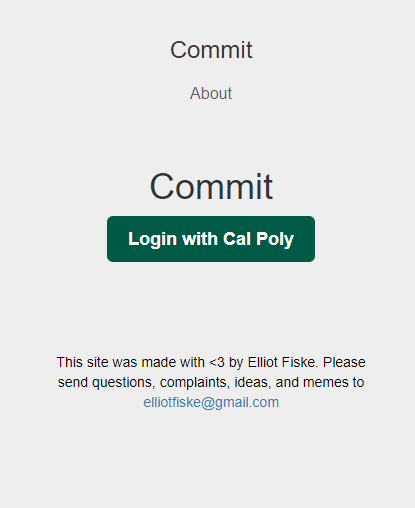
\includegraphics{figures/onboarding1}
	\caption{The login screen for \textit{Polycommit}, shown if the user does not have an active session.}
	\label{fig:onboarding1}
\end{figure*}

\par After clicking the login button, users are brought to the main Cal Poly login portal screen. Observant users will note that the callback URL points to \newline \textbf{https://users.csc.calpoly.edu/\textasciitilde{}efiske/login.php}. This is because the Cal Poly authentication service only will successfully make an authentication callback to a website on Cal Poly ITS' whitelist. In order to enable Cal Poly login, we had to implement a PHP script on the Cal Poly Unix servers' \textbf{www} directory that redirected to the Cal Poly portal, then handled the response.

\begin{figure*}[h]
	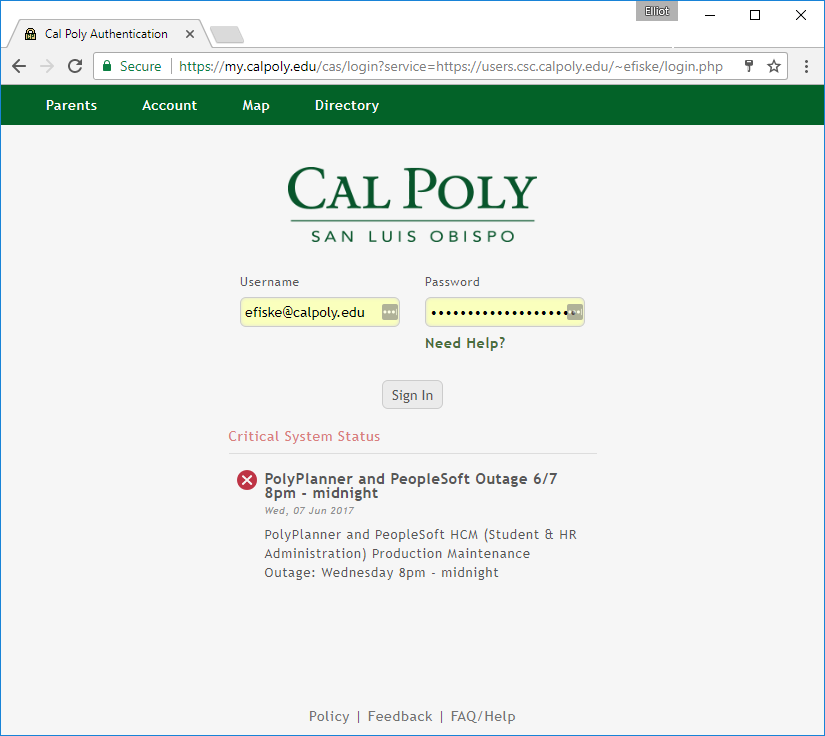
\includegraphics[width=1.0\linewidth]{figures/onboarding-portal}
	\caption{The main Cal Poly login portal. Note the URL that links back to my personal department folder.}
	\label{fig:onboarding1}
\end{figure*}

\par The full process for authentication is visible in \textbf{\hyperref[fig:logindiagram]{Figure \ref*{fig:logindiagram}}}. The user is redirected to Cal Poly's portal, which returns a \textbf{ticket}. That ticket is then passed to the \textit{Polycommit} backend and verified via a HTTP call from the \textit{Polycommit} server. Note that the ticket is only valid for the \textit{Polycommit} service; if a ticket is compromised, no user data is endangered and an attacker can not log in to any other Cal Poly-based service.

\par Once the ticket is verified on the backend, the user's session is created on the backend and the server responds with a session cookie.

\par The first time the user logs into \textit{Polycommit}, they are presented with a legal disclaimer describing the nature of the study. The full text of the disclaimer is available in \textbf{\hyperref[appendix:disclaimer]{Appendix \ref*{appendix:disclaimer}}}. Users will be redirected back to this disclaimer if they don't click the check mark to verify that they agree to the disclaimer. That is, even if the user tries to access a course page via URL, they will be sent back to the disclaimer until it is verified by the backend.

\begin{figure*}[h]
	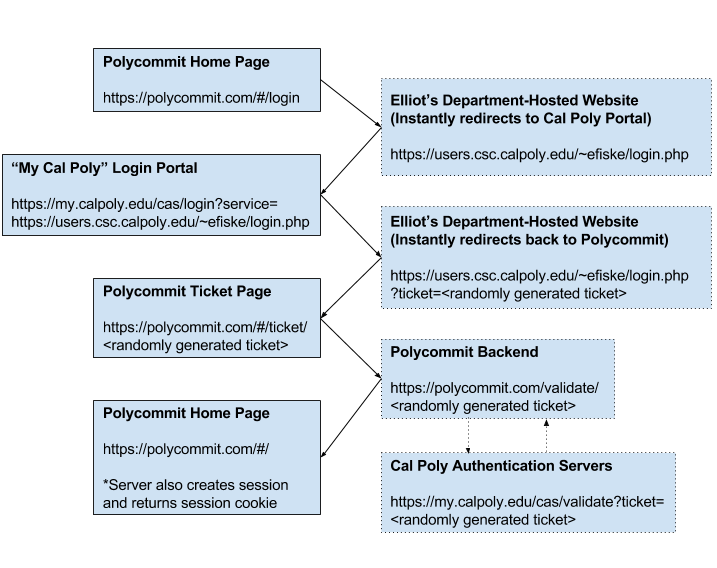
\includegraphics[width=1.0\linewidth]{figures/logindiagram}
	\caption{A diagram explaining how the Cal Poly authentication is handled on the backend. Sites that the user sees in their browser window have a solid outline, and sites that the user does not see are outlined in dotted lines. Similarly, network calls made by the user's computer are represented by a solid arrow, and network calls made by the \textit{Polycommit} backend are represented by a dotted arrow.}
	\label{fig:logindiagram}
\end{figure*}


\subsection{Home Screen}
\par Upon logging in, students click ``Enroll'' for the classes they wish to participate in. Upon enrolling, the classes are listed under the ``Enrolled Classes'' section (\textbf{\hyperref[fig:polycommit1]{Figure \ref*{fig:polycommit1}}}). This page also lists the two main ``scores'' that students earn by answering questions: \textbf{commitment} and \textbf{points}.

\par Commitment is a numerical value that represents how many \textit{unique} days a student has answered a question on the website. Students could earn up to 1\% extra credit on their final grade in the class by getting 15 commitment.

\par Points are earned by answering questions. More points are awarded for correct answers, and bonus points are awarded based on the user's current commitment. All participants in the experiment were placed in a raffle for \$20 Amazon gift cards. Additional entries into the raffle were awarded by earning more points.

\begin{figure*}[h]
	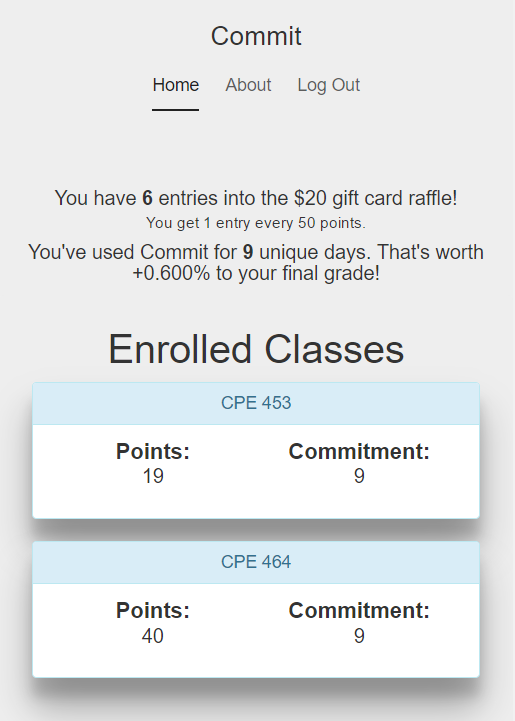
\includegraphics{figures/polycommit-screen}
	\caption{The ``Home'' screen for \textit{Polycommit}. Students can see their current progress and can click on a course to answer challenges.}
	\label{fig:polycommit1}
\end{figure*}

\subsection{Course Screen}
\par Each course page has a list of challenges (\textbf{\hyperref[fig:polycommit2]{Figure \ref*{fig:polycommit2}}}) that are open to the student. Challenges are grouped by the week in which they are opened. If a student has completed all the challenges in a week, the week is displayed with a green check mark and does not expand. If there are open challenges in a week, the week is displayed in yellow with an ``alert'' icon, indicating that the student has an available challenge. This UI imparts a sense of urgency to the user, since they could potentially lose opportunities to earn commitment by not answering a question in a 24-hour period. Each challenge also lists the date it was opened, and the number of points awarded if the challenge is already completed.

\par Finally, the Course page lists the student's points and commitment for the course, along with a tooltip that explains what ``commitment'' is. The commitment and point values are repeated from the home page since they are central to the experience of the app, and it is inherently satisfying to watch your points and commitment rise as you complete challenges.

\begin{figure*}
	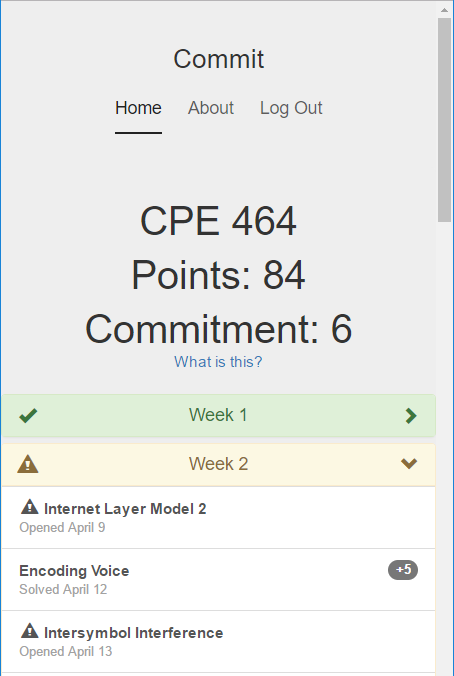
\includegraphics{figures/polycommit-challenges}
	\caption{The ``course'' screen for \textit{Polycommit}. Students can see their current points and commitment and can see a list of challenges organized by date.}
	\label{fig:polycommit2}
\end{figure*}

\subsection{Challenge Screen}
\par The challenge screen is where students see the content of a challenge and input their answers. A challenge can either be multiple choice, short answer, or numerical. An example of a simple multiple choice challenge is at \textbf{\hyperref[fig:polycommit3]{Figure \ref*{fig:polycommit3}}}.

\par At the bottom of the challenge screen is a link to submit feedback about a question. Through this link, students are brought to a Google form where they can provide feedback about a particular question. The feedback form is viewable at \textbf{\hyperref[fig:polycommit4]{Figure \ref*{fig:polycommit4}}}.

\par The question feedback form was not utilized as frequently as the other feedback forms. Only 2 responses came in through this form.

\par Once the challenge is closed, students can see a list of their previous attempts along with the correct answer to the problem. Certain problems have their answers hidden; for instance, all Linear Analysis problems don't show their answers because many challenges on \textit{Polycommit} are directly from the assigned homework. Hiding the correct answer prevents students from quickly inputting a wrong answer to see the homework solutions. Additionally, if a question has received feedback as being confusing, an ``Explanation'' field provides detailed context about the answer the problem and potential pitfalls (See  \textbf{\hyperref[fig:polycommit5]{Figure \ref*{fig:polycommit5}}}).

\begin{figure*}
	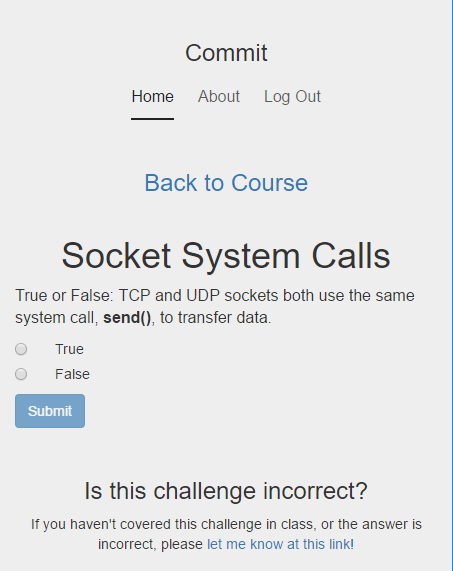
\includegraphics{figures/pc-question}
	\caption{The ``Challenge'' screen for Polycommit. Students see the content of the challenge and can enter their answers. At the bottom is a link where students can give feedback on a challenge.}
	\label{fig:polycommit3}
\end{figure*}


\begin{figure*}
	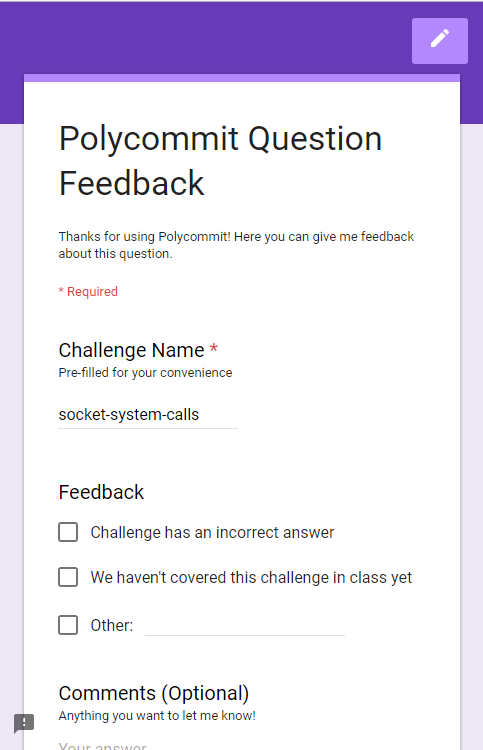
\includegraphics{figures/pc-feedback}
	\caption{The Feedback form for questions. The id for the question is automatically filled in. The student can optionally enter their email address (off-screen) if they want to be contacted when the challenge is fixed.}
	\label{fig:polycommit4}
\end{figure*}

\begin{figure*}
	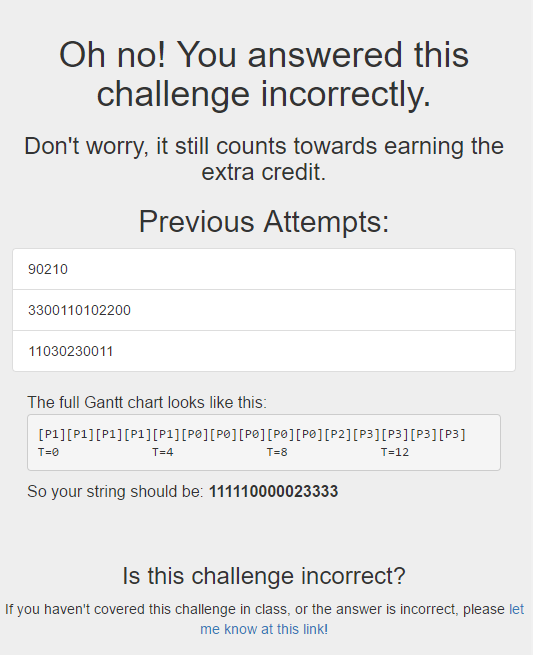
\includegraphics{figures/pc-incorrect}
	\caption{The view of a challenge once it has been answered incorrectly. The main message assures the user that it still counts for commitment. A full explanation of the problem is under the list of the user's attempts.}
	\label{fig:polycommit5}
\end{figure*}

\subsection{Toasts}
\par \textit{Polycommit} uses ``toasts'' to convey temporary, state-based information to the user. For instance, when the user answers a question, they get immediate feedback in the form of a pop-up toast. Positive information, such as a correct answer, is styled with a green background and a check mark. Negative information, such as an incorrect answer or a server error, is bright red with an alert symbol that commands the user's attention. Examples of each are at \textbf{\hyperref[fig:polycommit6]{Figure \ref*{fig:polycommit6}}}.


\begin{figure*}
	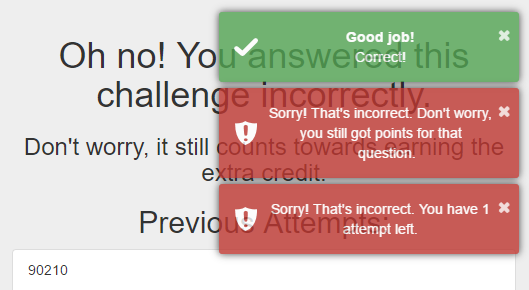
\includegraphics{figures/pc-toast}
	\caption{Three examples of ``toast'' notifications. These provide useful state-based information, such as whether a challenge was answered correctly. They also can provide feedback if an error occurred, such as a challenge not submitting due to poor network connectivity.}
	\label{fig:polycommit6}
\end{figure*}

\section{User Rewards}

\par In order to incentivize students to use \textit{Polycommit}, we introduced two main rewards for participation.

\subsection{Extra Credit}

\par We made an agreement with the instructor of each course that a small amount of extra credit would be offered to students that made use of \textit{Polycommit}. In order to make the UI uniform for all users, we introduced the same reward for all users: 1\% extra credit added to the student's final score in the class for earning 15 commitment. If students earned less than 15 commitment, they received a percentage of the extra credit proportionate to their commitment value. No additional credit was awarded for earning more than 15 commitment.

\par The experiment ran for 5 weeks, giving users ample time to reach this goal. The extra credit proved to be a strong motivator for participation, as several students contacted me about receiving the extra credit throughout the quarter.

\par We chose to offer extra credit for earning commitment rather than points, because we were more interested in students using the app consistently than rewarding correct answers.

\subsection{Amazon Gift Card Drawing}

\par In addition to the extra credit, we ran a raffle for 8 \$25 Amazon gift cards. Students earn one additional entry into the raffle for every 50 points they earn using \textit{Polycommit}. Students are reminded of the raffle on the home screen, where the number of raffle entries they had earned so far is displayed prominently across the top.

\par In order to maintain the legality of the raffle, any Cal Poly student could also send me an email every week to receive an entry into the raffle. This was described in the disclaimer students read upon signing up for the experiment. No such emails were received throughout the duration of the experiment.

\section{Technology Used}
\par All the code for \textit{Polycommit} is available here:
\hyperref[https://github.com/elliotfiske/commitment]{https://github.com/elliotfiske/commitment}

\par \textit{Polycommit} has its origins in a Summer 2016 section of Dynamic Web Development (CPE 437), taught by Dr. Clint Staley. The base code and overall code architecture remain, as well as some of the platforms used. The app runs on a M*EAN stack. It uses Node.js as a backend, with Express as a routing service and MySQL as a database. In addition, Sequelize is used to easily interface with the database from Javascript. Angular.js is used as a frontend framework, supplemented by Bootstrap for reactive layout.

\par Node.js and Javascript lends itself well to quick, iterative development. As a dynamically typed language with first-class and anonymous functions, it is easy to quickly make sweeping changes based on user feedback. However, since Javascript is an interpreted language, potential errors that a compiler could have caught may make it through to the live site. Because of this, it was extremely important to regularly run the backend code through comprehensive unit tests.

%\subsection{HTTPS}
%\par In order to %TODO: Talk about how HTTPS builds user trust and encourages them to enter their credentials.

\subsection{Test-First Methodology}
\par All of the backend server code is thoroughly covered by various test cases. We used the service \textit{Postman} to maintain a suite of tests that ensured all the data involved in \textit{Polycommit} was both available and secure. \textit{Postman} allows developers to run a series of web requests against a server, and verify that the correct response or error code is returned (See  \textbf{\hyperref[fig:postman]{Figure \ref*{fig:postman}}}). For instance, one test suite logs in as a student and attempts to complete a challenge, create a class, and query the information of another student. Only the first request should complete successfully; the student's unprivileged account should not be able to create classes or see other students' data.

\begin{figure*}
	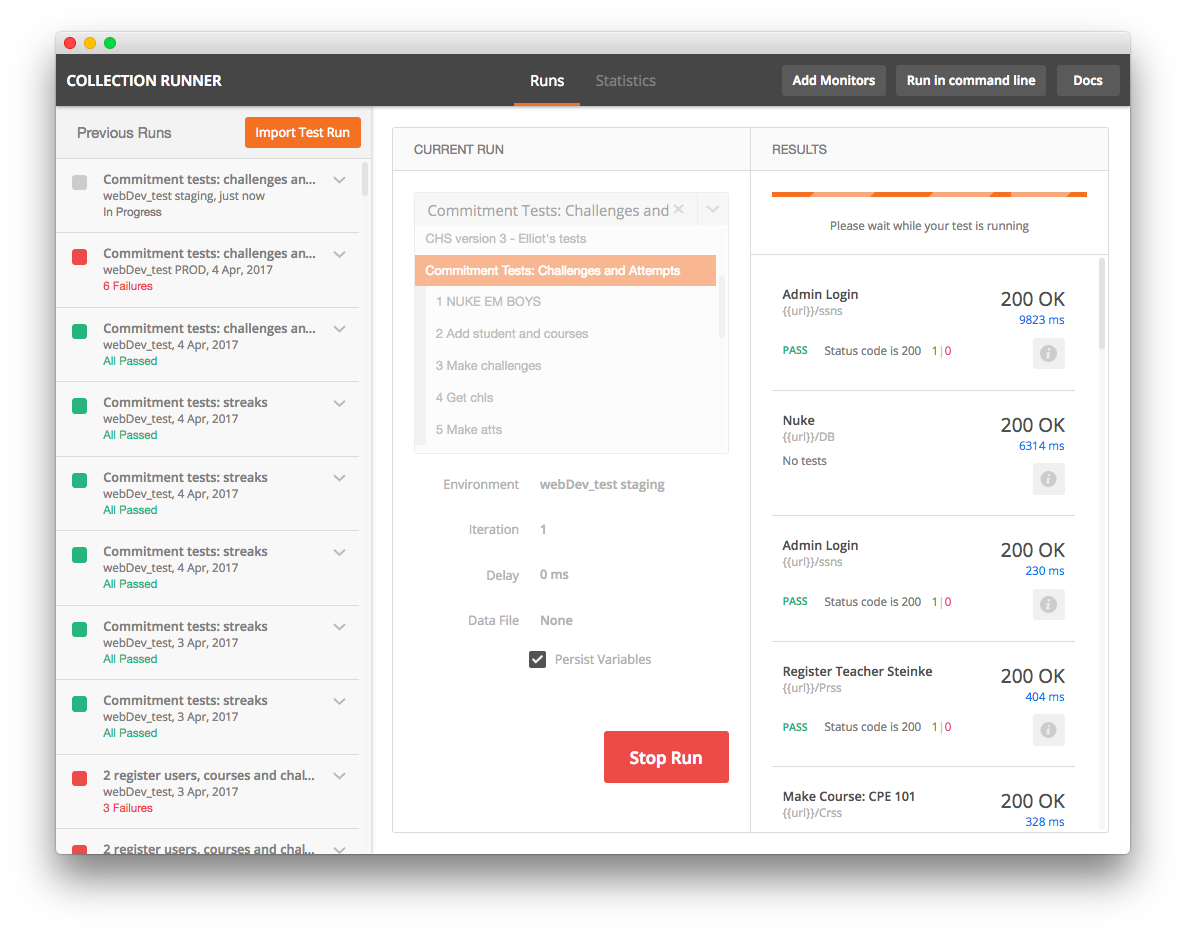
\includegraphics[width=1.1\linewidth]{figures/postman}
	\caption{The Postman interface. A series of web requests are sent to the website, and a series of conditions determine whether the tests pass or fail.}
	\label{fig:postman}
\end{figure*}

\par Writing test cases for new server functionality \textit{before} beginning development allowed me to see edge cases before they arose, and allowed for the satisfaction of seeing the tests pass as I completed each feature. In addition, it protected the privacy of students' answers and scores.



\section{User Feedback}
\par At the bottom of every page is a link encouraging users to send feedback to an email address (See \textbf{\hyperref[fig:feedbacklink]{Figure \ref*{fig:feedbacklink}}}). Throughout the experiment, we received a large amount of excellent feedback that helped me refine the app's usability.

\begin{figure*}
	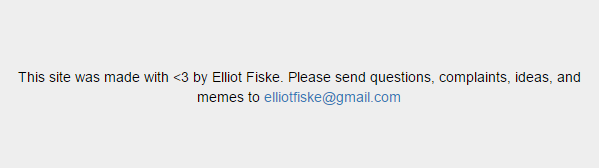
\includegraphics[width=1.1\linewidth]{figures/feedbacklink}
	\caption{The feedback link where students are encouraged to send feedback about \textit{Polycommit}.}
	\label{fig:feedbacklink}
\end{figure*}

\subsection{Early Testing}
\par Before the main experiment in Spring 2017 term, we ran a small dry run of the app to get a general feel for usability issues. The app was announced in CPE 464 in week 6, directly after the midterm. The main difference from the final iteration is the onboarding process. Instead of registering and logging in through the Cal Poly portal, students registered using an email address and had to click a link that was emailed to them to complete registration.

\par We discovered that this onboarding process had an extremely high drop-off rate. Of the 10 people that visited the posted link, only 4 entered their email, and only 2 successfully completed registration. As such, it became a huge priority to reduce the number of steps a user had to complete to begin using the app. The Cal Poly authentication process described above decreased the number of steps the user needed to take to enter the app, and thus gave a huge boost to user engagement.
